\documentclass[pdflatex,sn-vancouver-num]{sn-jnl}
\usepackage{graphicx}
\usepackage{amsmath,amssymb}
\usepackage{xcolor}
\usepackage{url}
\raggedbottom
\renewcommand{\figurename}{Supplementary Figure}
\renewcommand{\thefigure}{S\arabic{figure}}

\begin{document}

\title[Supplementary information]{Supplementary information: Spatial association of TLS programs and LAMP3\texorpdfstring{$^{+}$}{+}CCR7\texorpdfstring{$^{+}$}{+} mregDC states marks an immune-prognostic context in ovarian cancer}
\author[1]{\fnm{Feifan} \sur{Lu}}
\author[2]{\fnm{Ting} \sur{Zhang}}
\author*[1]{\fnm{Rui} \sur{Guan}}\email{cngreen785@163.com}
\author*[1]{\fnm{Mingjuan} \sur{Xu}}\email{mingjuanxu@smmu.edu.cn}
\affil[1]{\orgdiv{Department of Obstetrics and Gynecology}, \orgname{Changhai Hospital, Naval Medical University}, \orgaddress{\city{Shanghai}, \postcode{200433}, \country{China}}}
\affil[2]{\orgdiv{Department of Hematology}, \orgname{Shanghai East Hospital, Tongji University}, \orgaddress{\city{Shanghai}, \postcode{200120}, \state{Shanghai}, \country{China}}}
\maketitle

\section*{Supplementary Figure Legends}

\begin{figure}[ht]
\centering
\makebox[\textwidth][c]{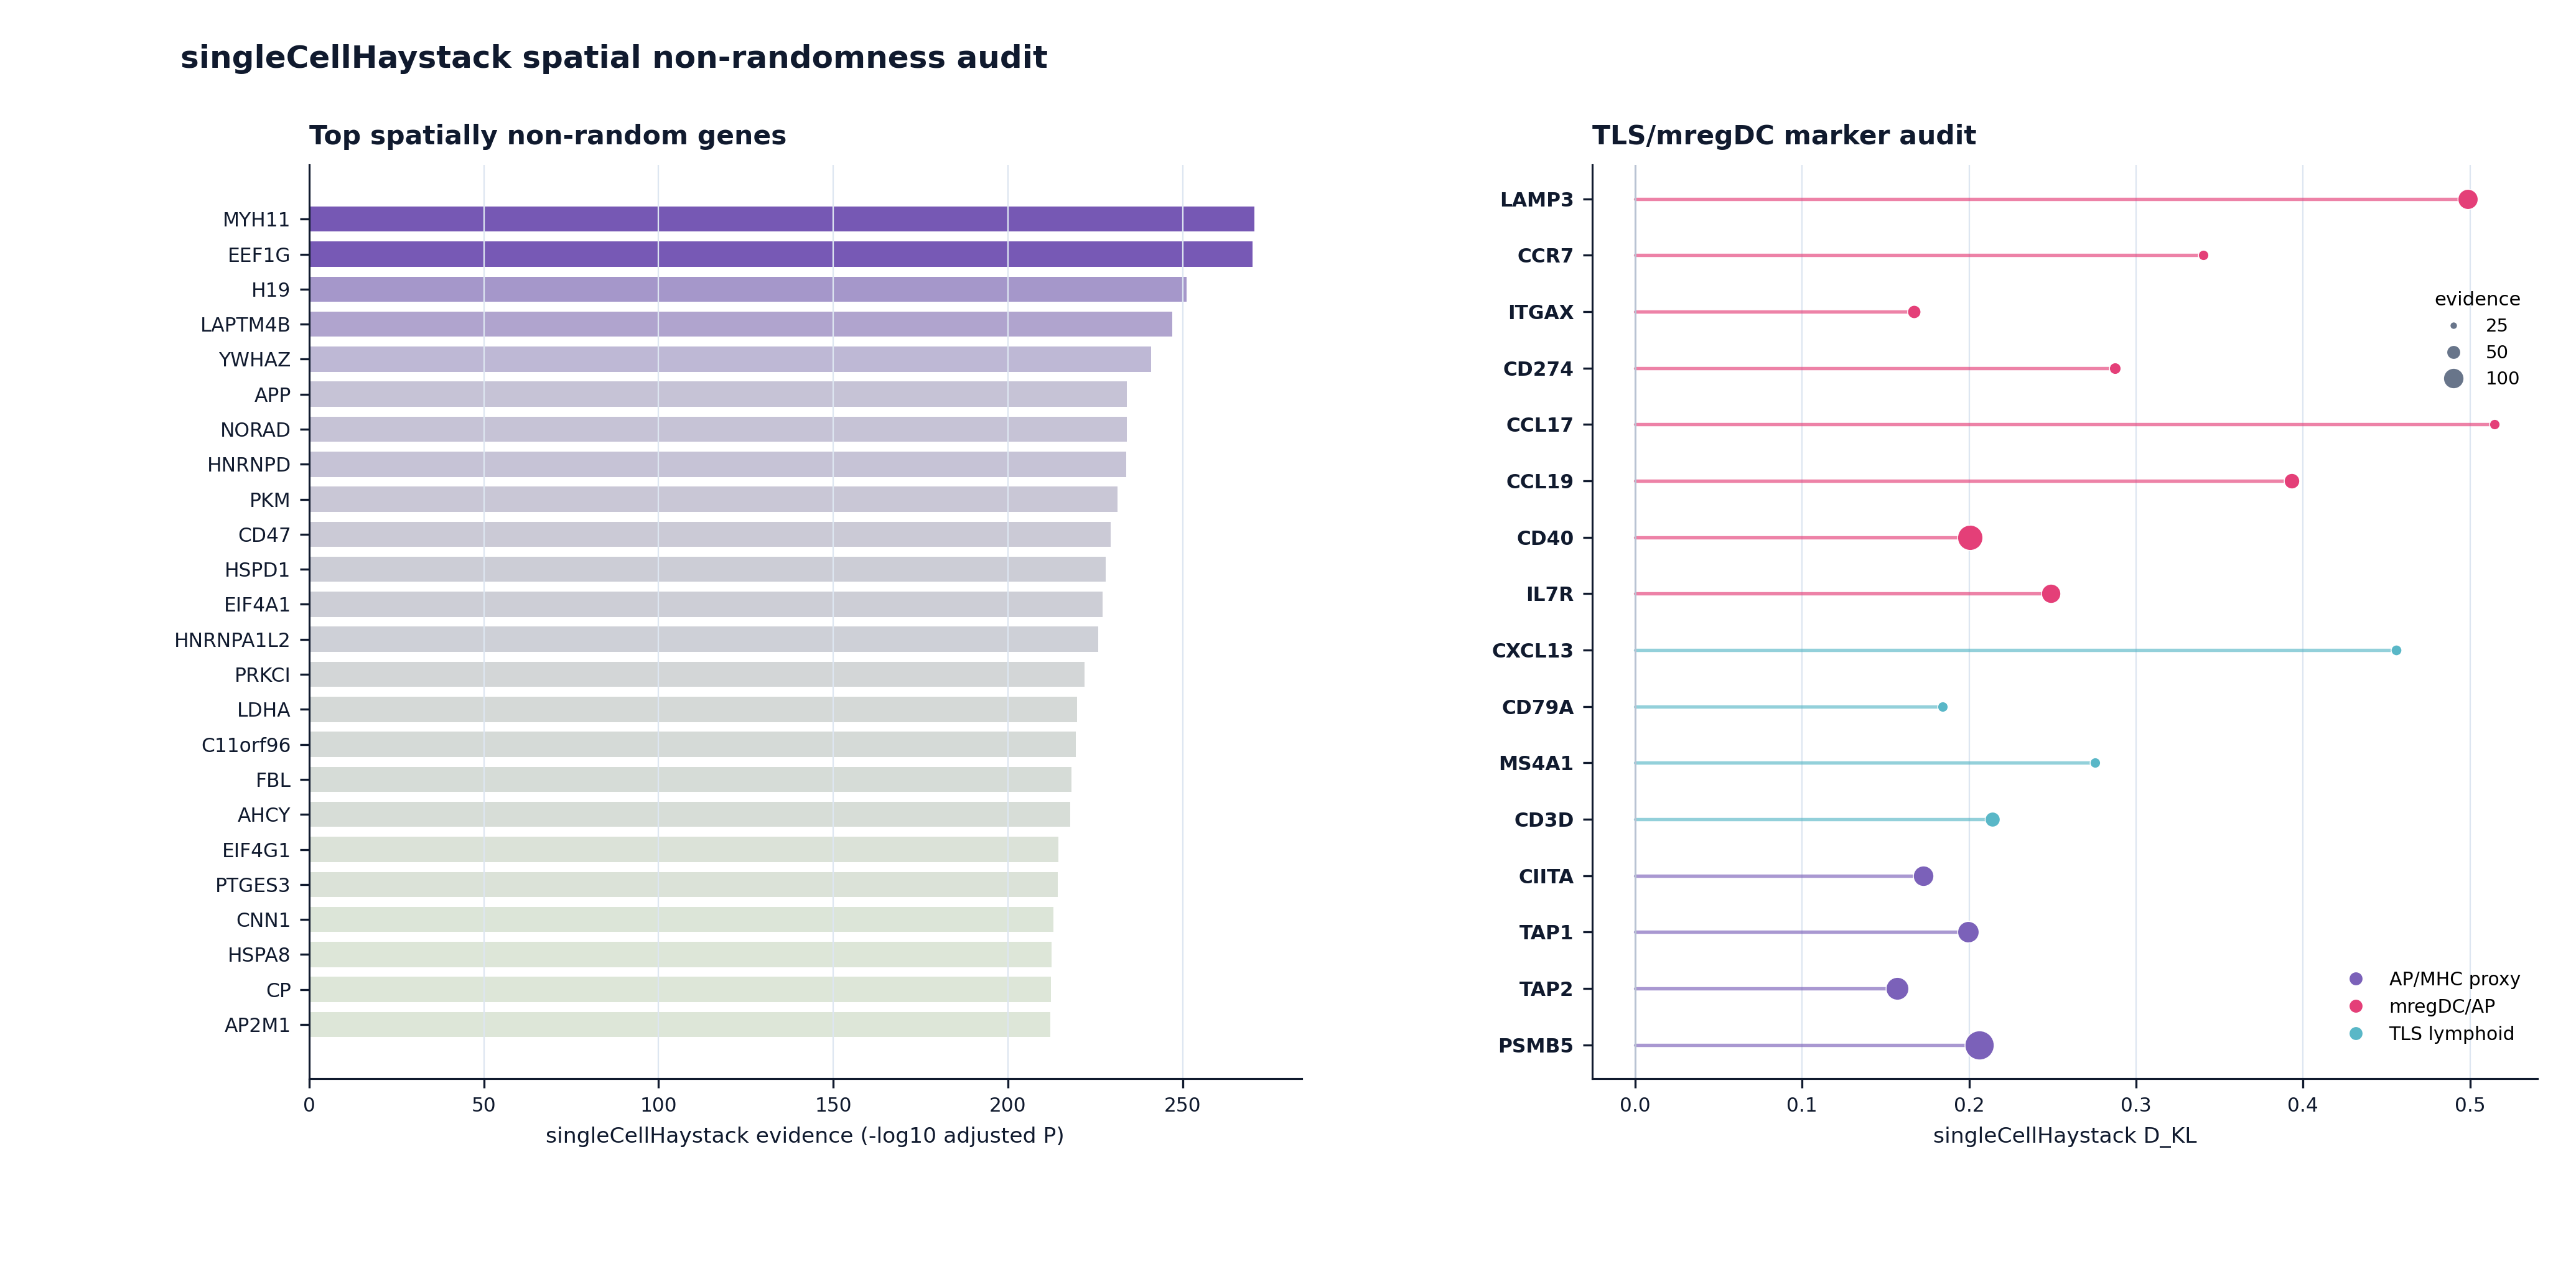
\includegraphics[width=372pt]{FigureS1_singleCellHaystack.png}}
\caption{\textbf{singleCellHaystack spatial non-randomness audit.} Ranked Xenium genes and marker-level evidence summarize spatially non-random transcriptional features in the deterministic ovarian cancer subset.}
\label{figS1}
\end{figure}
\clearpage

\begin{figure}[ht]
\centering
\makebox[\textwidth][c]{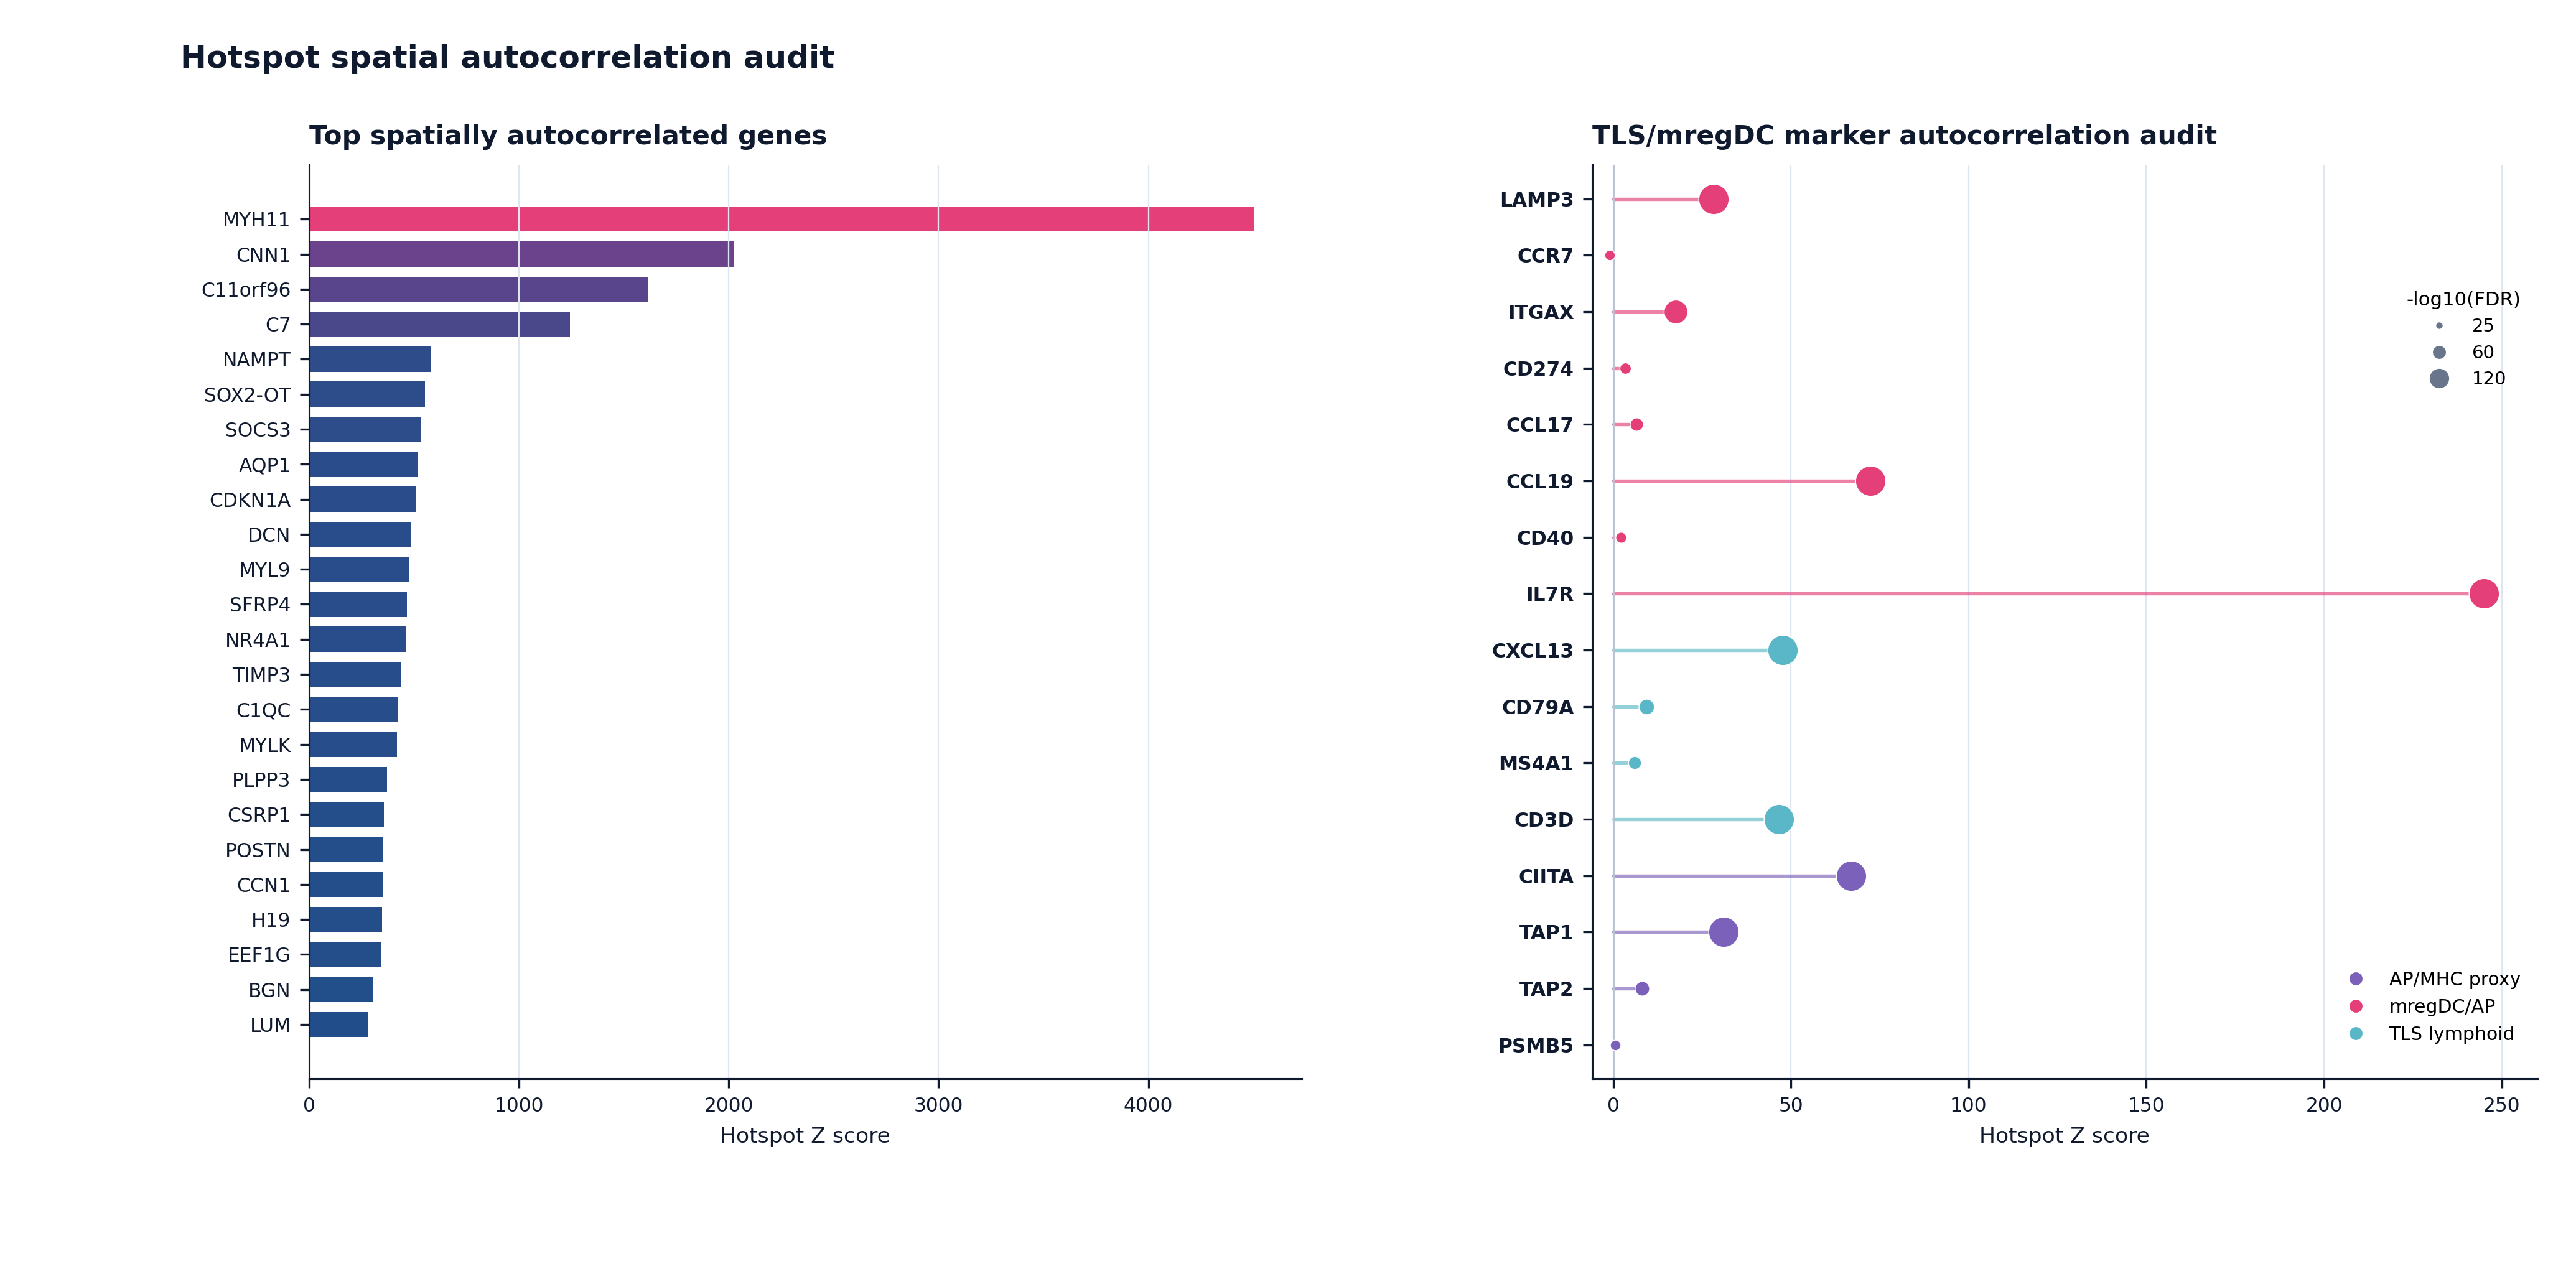
\includegraphics[width=372pt]{FigureS2_Hotspot.png}}
\caption{\textbf{Hotspot spatial-autocorrelation audit.} Ranked Xenium genes and marker-level Hotspot statistics summarize spatial autocorrelation of TLS/mregDC/antigen-presentation-associated features.}
\label{figS2}
\end{figure}
\clearpage

\begin{figure}[ht]
\centering
\makebox[\textwidth][c]{
\includegraphics[width=372pt]{FigureS3_Xenium_spatial_maps-re.pdf}}
\caption{\textbf{Xenium spatial maps supporting feature audits.} Module maps, non-random gene-expression maps, TLS-score alignment, co-high cells, and Hotspot representative genes are shown in the same spatial coordinate framework.}
\label{figS3}
\end{figure}
\clearpage

\begin{figure}[ht]
\centering
\makebox[\textwidth][c]{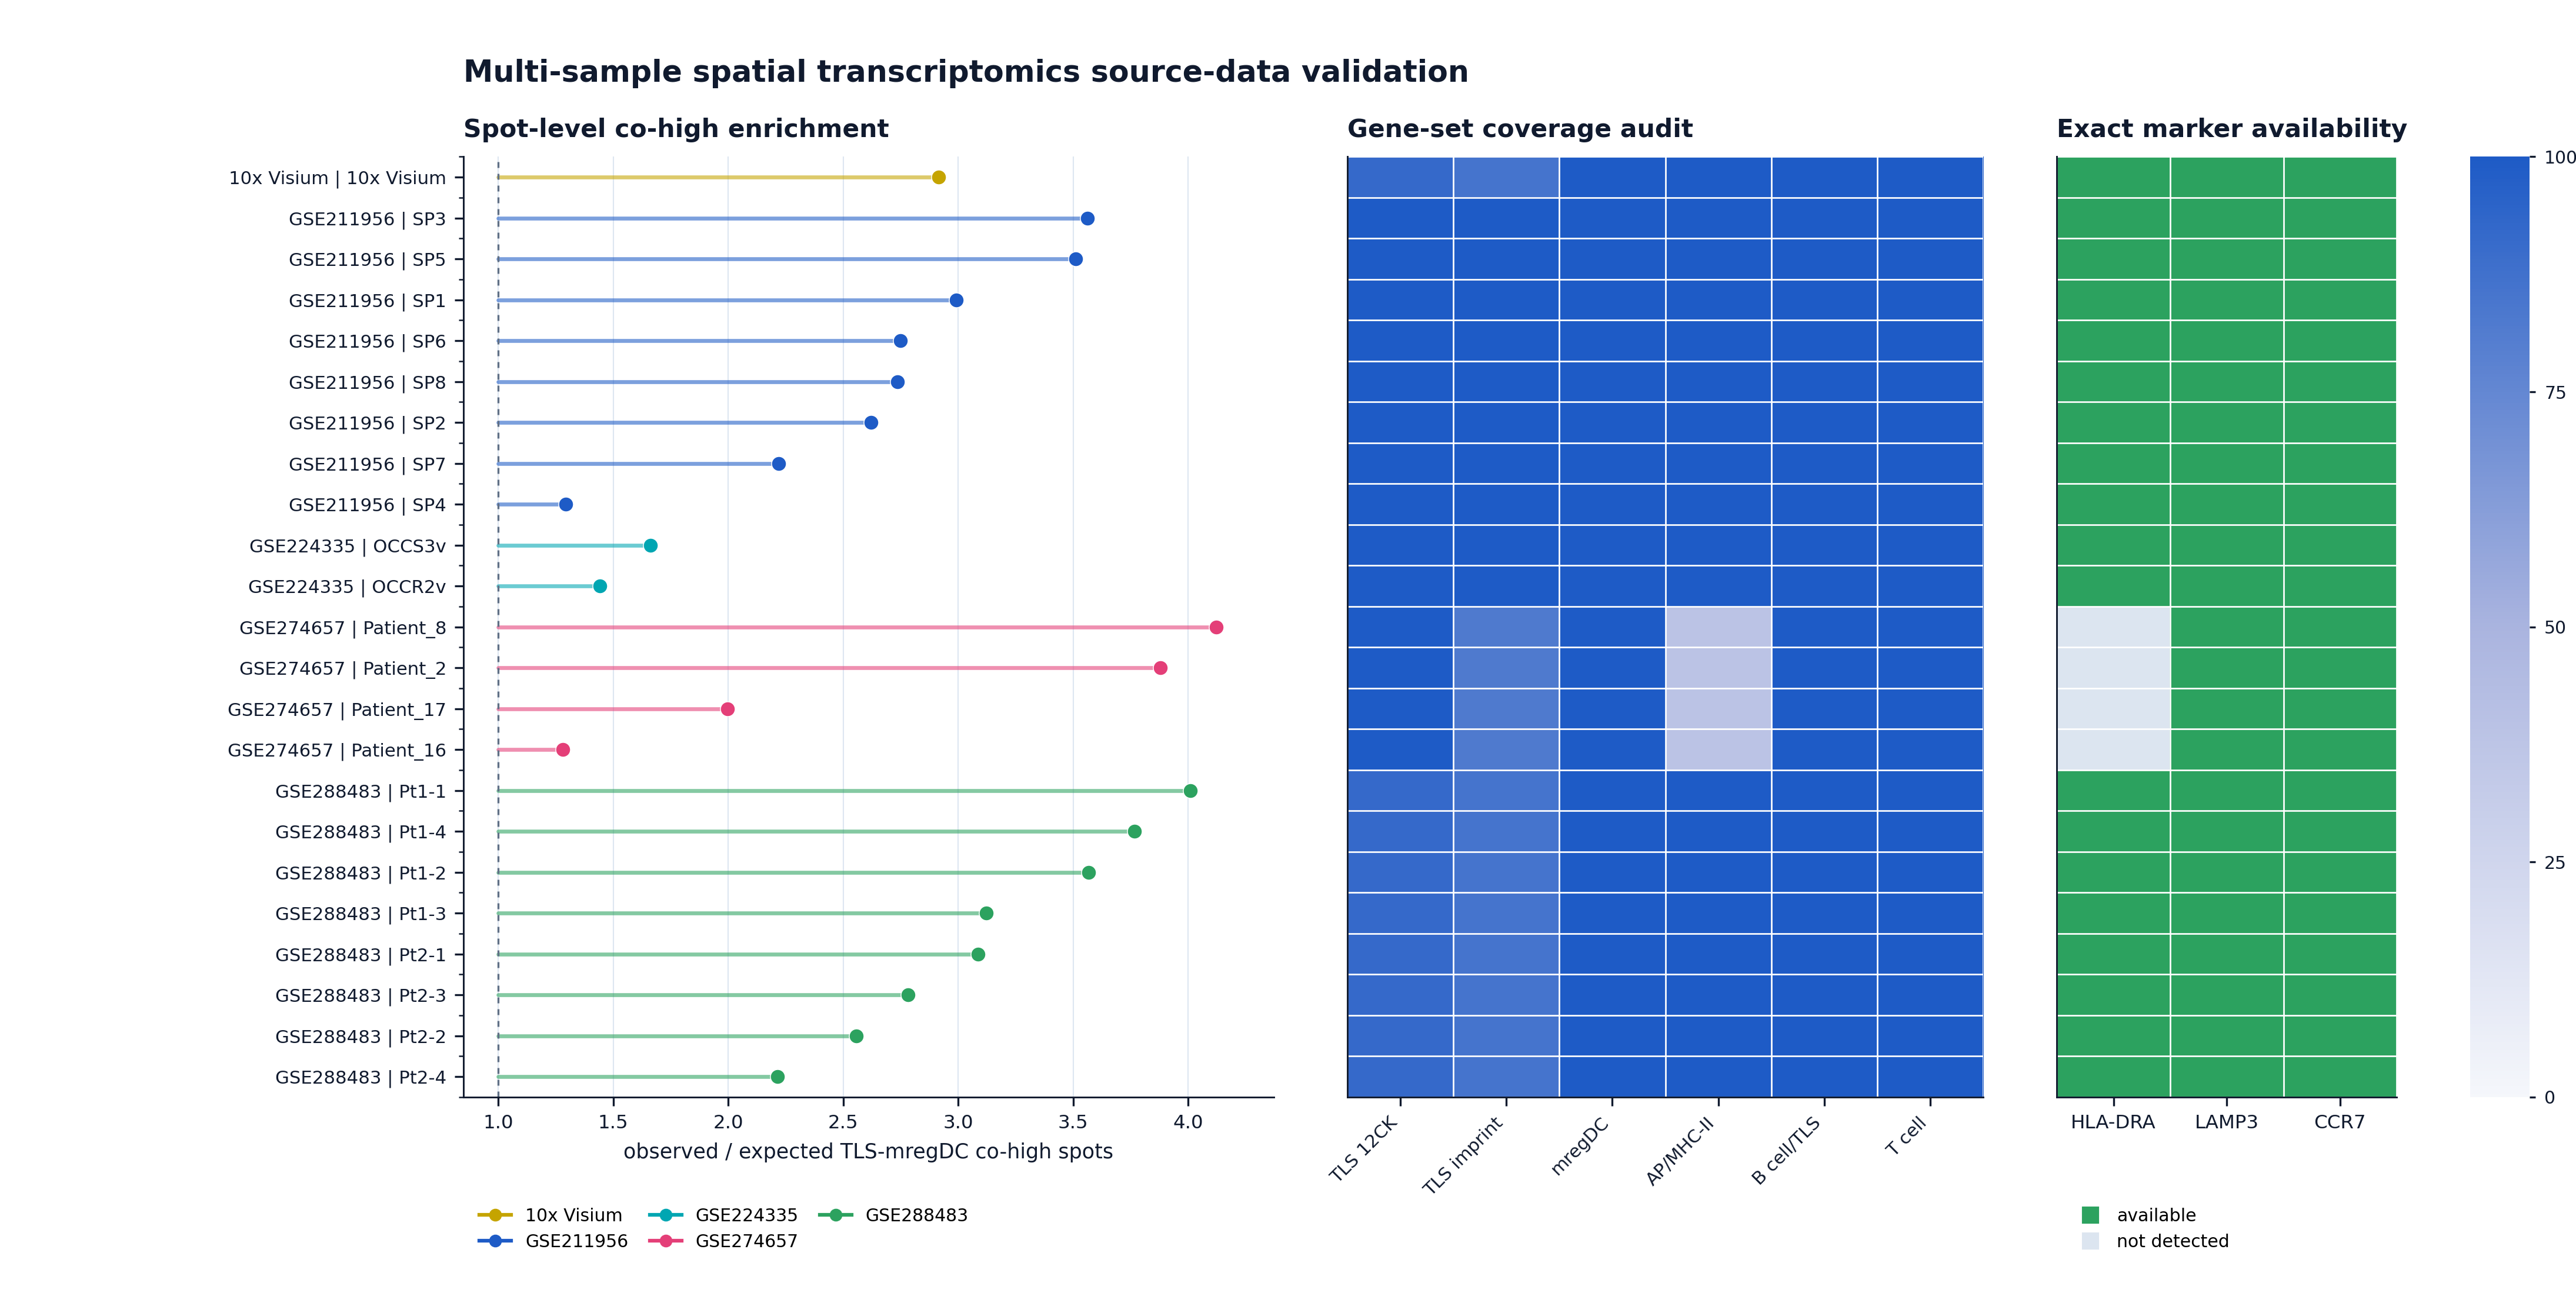
\includegraphics[width=372pt]{FigureS4_multi_sample_spatial_validation.png}}
\caption{\textbf{Expanded multi-sample spatial source-data validation.} Spot-level co-high enrichment, gene-set coverage, and exact-marker availability summarize public ovarian spatial datasets used for Fig.~5.}
\label{figS4}
\end{figure}
\clearpage

\begin{figure}[ht]
\centering
\makebox[\textwidth][c]{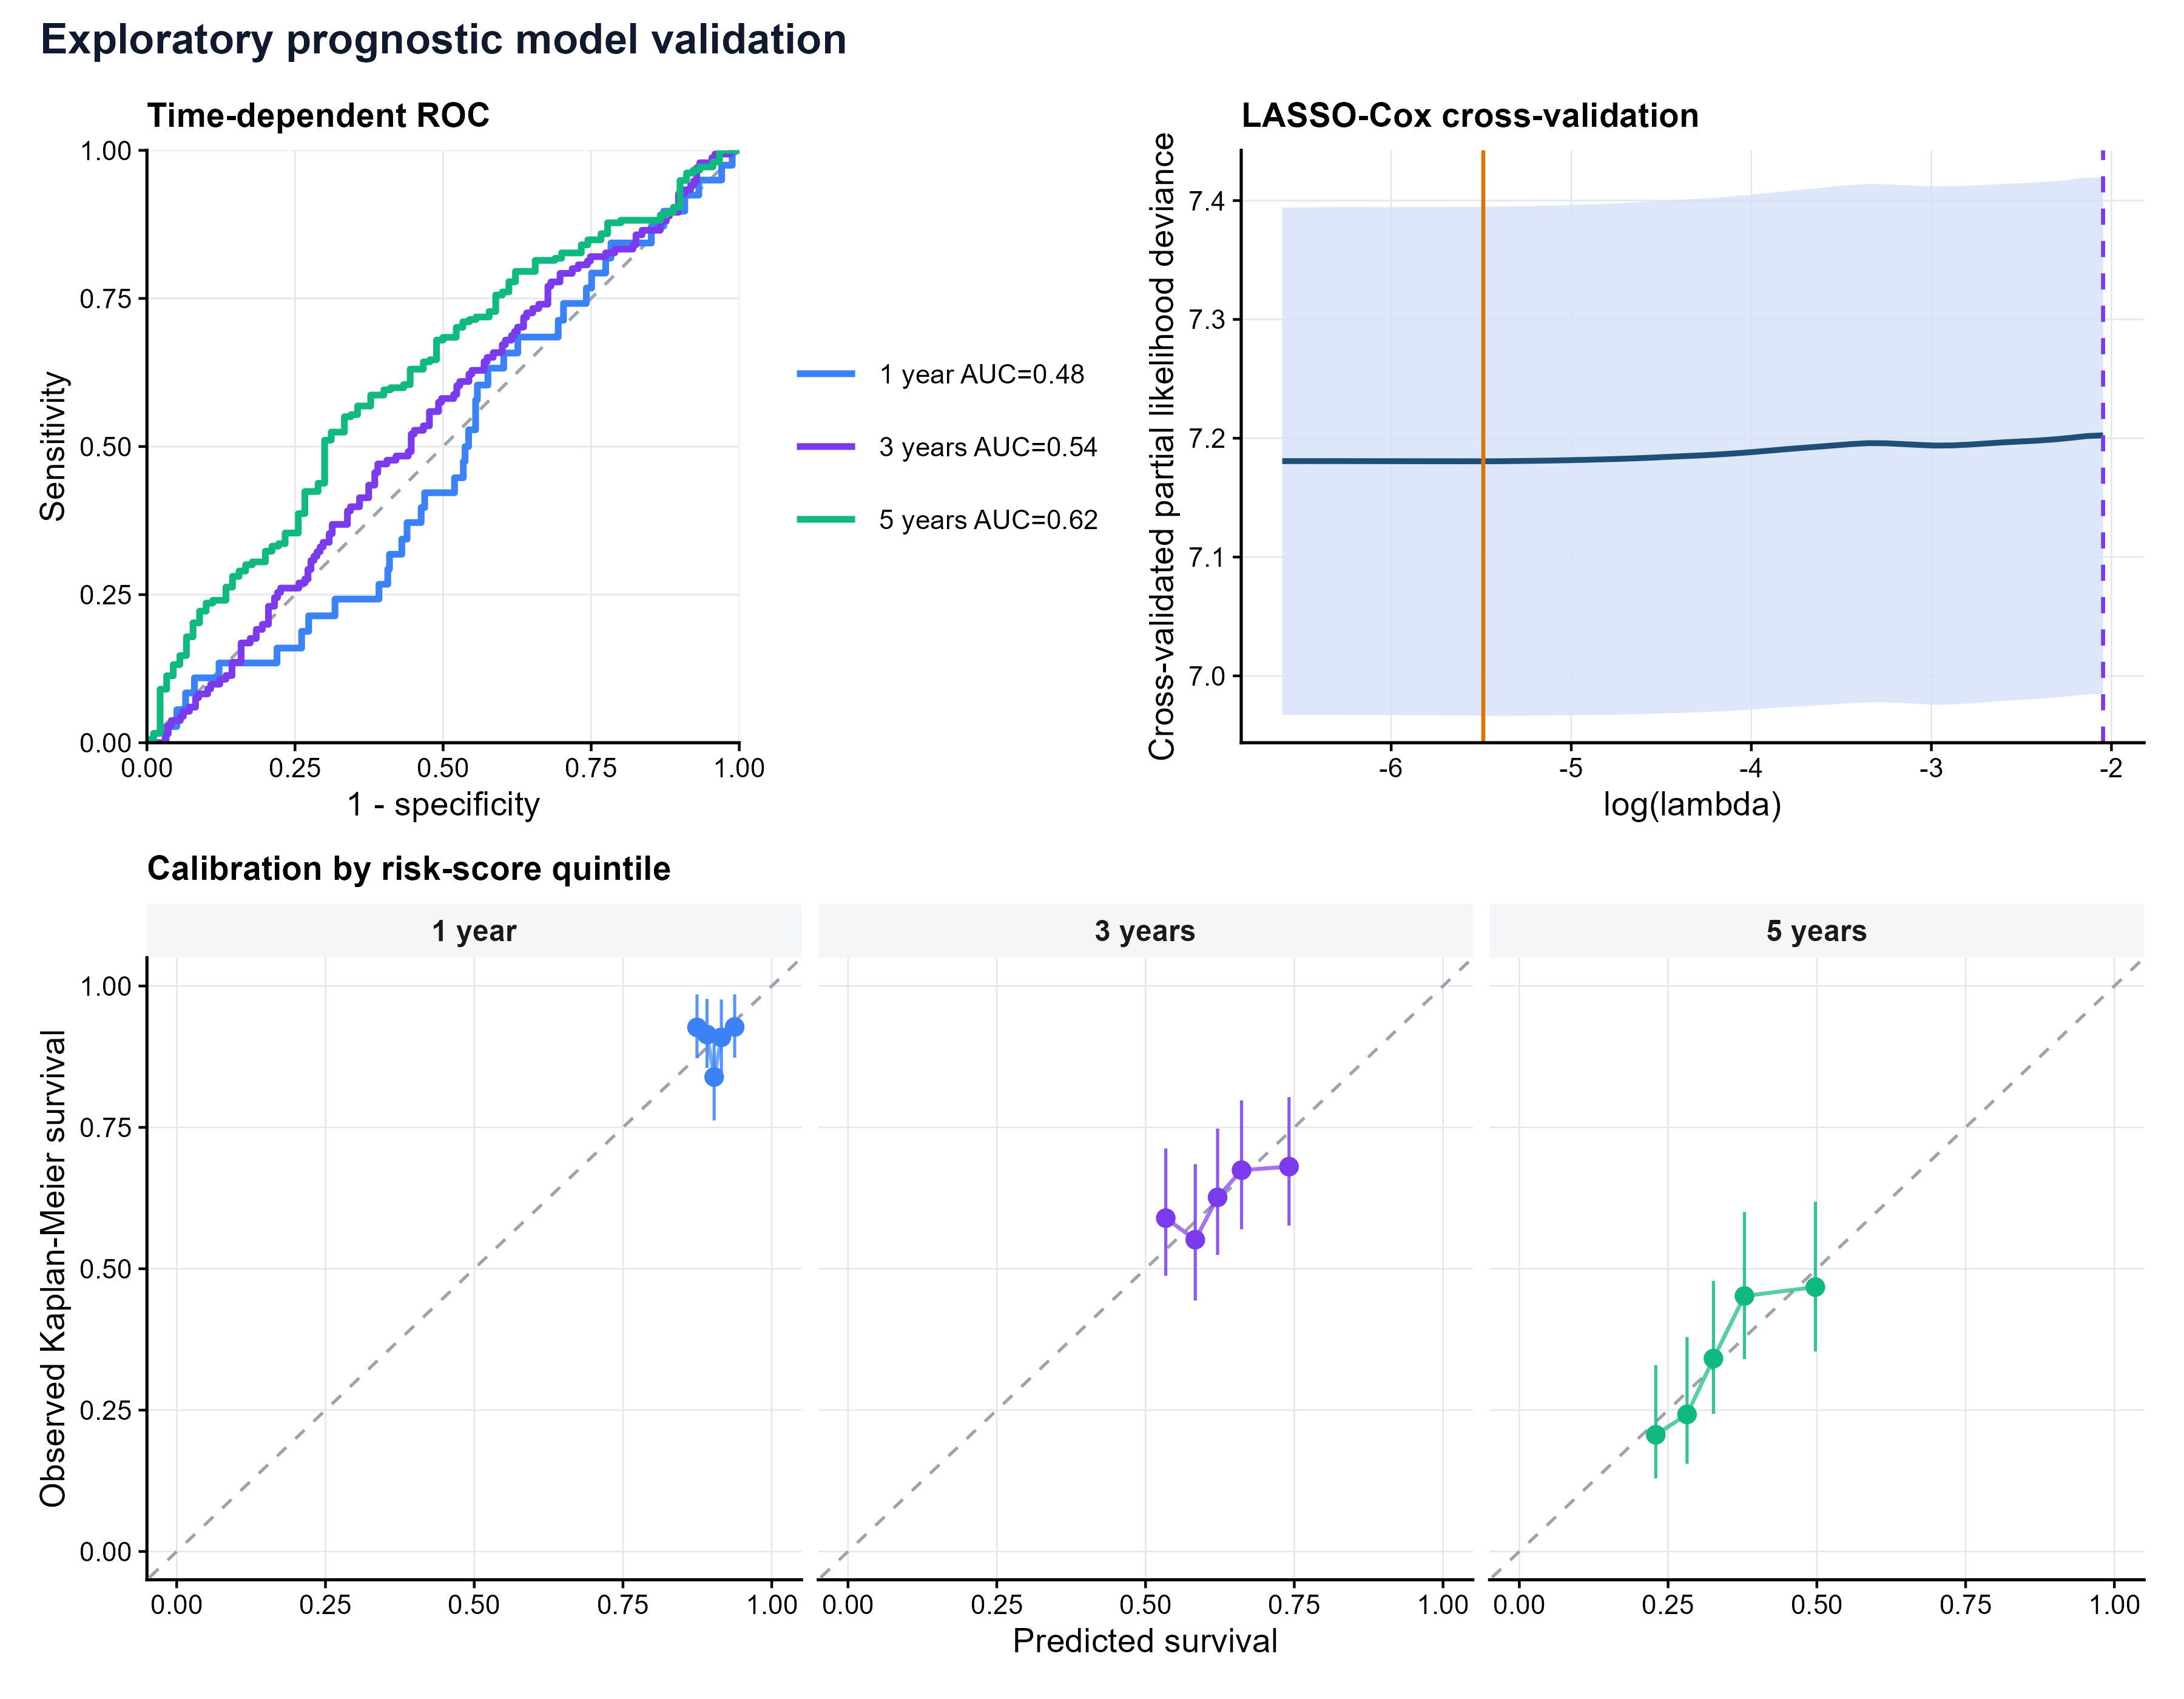
\includegraphics[width=372pt]{FigureS5_model_validation.png}}
\caption{\textbf{Exploratory model validation.} Time-dependent ROC, LASSO-Cox cross-validation, and calibration-by-risk-quintile summaries support internal assessment of the TCGA-OV exploratory model.}
\label{figS5}
\end{figure}
\clearpage

\begin{figure}[ht]
\centering
\makebox[\textwidth][c]{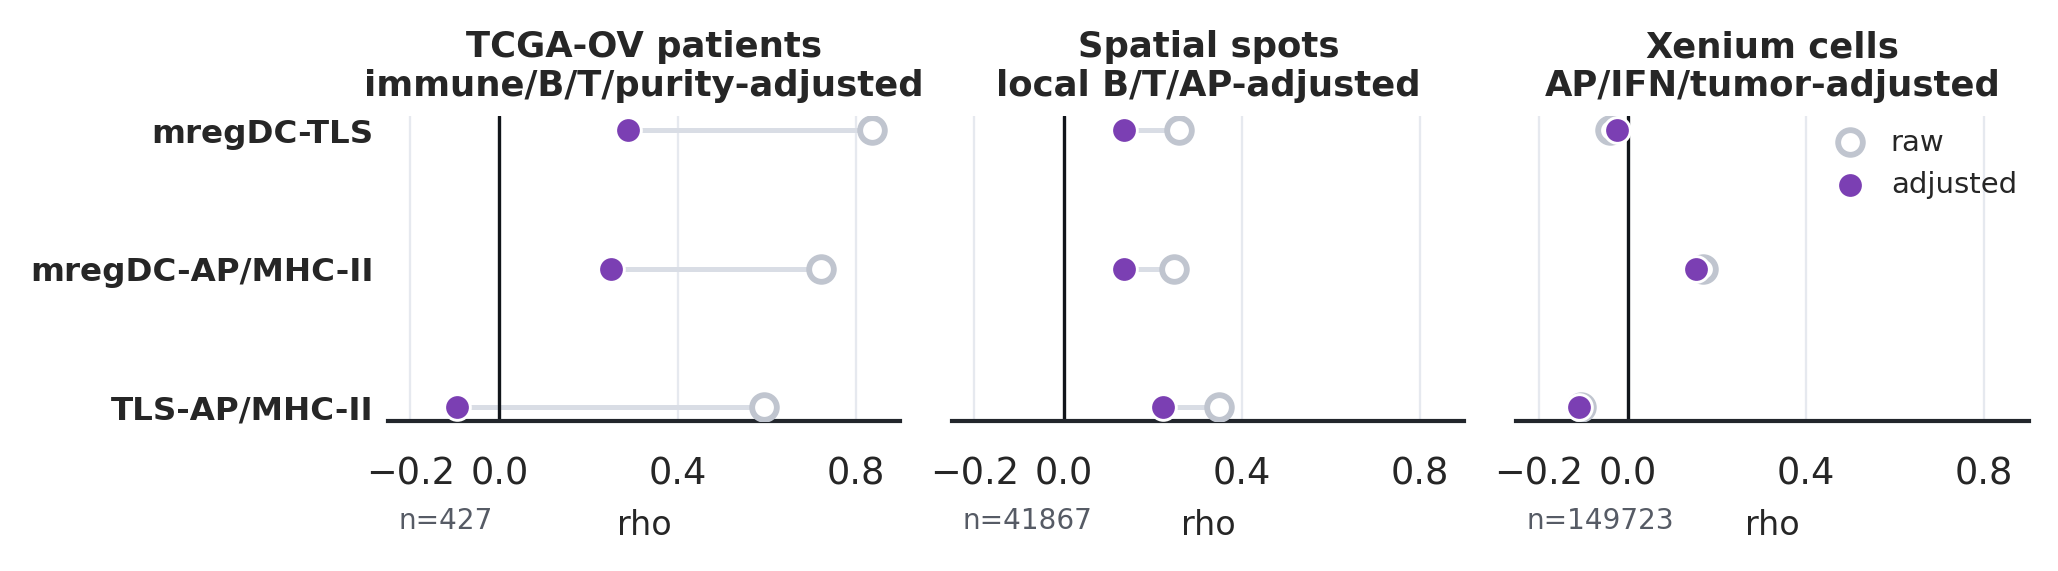
\includegraphics[width=372pt]{FigureS6_specificity_adjusted_associations.png}}
\caption{\textbf{Immune-richness-adjusted specificity audit.} Raw and adjusted Spearman correlations summarize TCGA-OV patient-level, multi-sample spatial, and Xenium sensitivity analyses for mregDC/TLS/AP associations.}
\label{figS6}
\end{figure}
\clearpage

\section*{Supplementary Source Data}
\begin{itemize}
\item Current-numbering source-data map for main and supplementary figures: \texttt{source\_data/SOURCE\_DATA\_INDEX.csv}.
\item Fig. S1: \texttt{source\_data/FigS01\_singleCellHaystack\_audit}.
\item Fig. S2: \texttt{source\_data/FigS02\_Hotspot\_audit}.
\item Fig. S3: \texttt{source\_data/FigS03\_Xenium\_spatial\_maps}.
\item Fig. S4: \texttt{source\_data/FigS04\_multi\_sample\_spatial\_source}.
\item Fig. S5: \texttt{source\_data/FigS05\_model\_validation}.
\item Fig. S6: \texttt{source\_data/FigS06\_specificity\_adjustment}.
\item Signature definitions, GEO source reconstruction, public spatial and 10x dataset accessions, and gene-coverage audits are provided in Supplementary Tables S1--S3 and \texttt{source\_data/Tables\_signature\_and\_GEO}.
\item Legacy source-data folders are retained for traceability but should be interpreted through the current-numbering index.
\end{itemize}

\section*{Supplementary Tables}
Supplementary Table S1 contains the reconstructed 22-sample scRNA-seq GEO source manifest, disease labels, sample counts, and accession-level summaries.

Supplementary Table S2 contains signature definitions, gene-coverage audits, marker-availability checks, and legacy-label harmonization for the mregDC, TLS, antigen-presentation/MHC-II, IFN, FDC/GC, HEV/stromal, proliferation, and EMT/invasion modules.

Supplementary Table S3 contains the 23 public multi-sample spatial transcriptomic samples used for Fig.~5/Fig.~S4, including one public 10x Visium ovarian FFPE sample within the 23-sample spatial set, dataset-level GSE identifiers, sample-level GSM identifiers where applicable, and spot/cell counts. The same table also lists the separate public 10x scFFPE and Xenium Prime ovarian cancer reference datasets with URLs and software-version notes.

\end{document}
